
\chapter{Leyes de Kirchhoff generalizadas}


\subsection{Productos $SU(2)$}
\begin{frame}[fragile,allowframebreaks]
Sean $A$ y $B$ $C$, dobletes $SU(2)$. En el Lagrangiano \eqref{eq:L0}, hemos construido invariantes $SU(2)$ de la forma $C^{\dagger}B$, por ejemplo. Pero hay otra forma de construir el producto invariante

Para los dobletes  $SU(2)_L$ 
\begin{align}
  A=&
  \begin{pmatrix}
    A^1\\
    A^2\\
  \end{pmatrix},&
  B=&
  \begin{pmatrix}
    B^1\\
    B^2\\
  \end{pmatrix},&
  C=&
  \begin{pmatrix}
    C^1\\
    C^2\\
  \end{pmatrix},
\end{align}
podemos definir un producto que es invariante bajo $SU(2)$ como el producto escalar bajo la ``métrica'' de $SU(2)$
\begin{align}
\epsilon^{ab}A_a B_b\to \epsilon_{ab}A'_a B'_b=&\epsilon_{ab}U_{ac}U_{bd}A_c B_d\nonumber\\
  =&\left( U_{11}U_{22}-U_{12}U_{21} \right)\left(A_1B_2-A_2B_1  \right)\nonumber\\
  =&\epsilon^{ab}\det\mathbf{U} A_a B_b\nonumber\\
  =&\epsilon^{ab} A_a B_b\,.
\end{align}
Teniendo en cuenta que
\begin{align}
  \epsilon^{ab}A_a B_b=&A_1 B_2-A_2 B_1 \,.
 \end{align}
Con el contenido de campos de $A$, siempre es posible definir un nuevo doblete adjunto de $SU(2)$, definido como 
\begin{align}
\label{eq:conjA}
 \widetilde{A}=& \begin{pmatrix}
                  A_2^{*}\\
                 -A_1^{*}\\
                \end{pmatrix}
\end{align}
En tal caso es posible escribir el producto escalar $SU(2)$ es una forma matricial, la cual muestra una invarianza más evidente
\begin{align}
\widetilde{A}\cdot B\equiv \epsilon^{ab}\widetilde{A}_a B_b=&\widetilde{A}_1 B_2-\widetilde{A}_2 B_1 \nonumber\\
                     =&A_2^{*}B_2 -(-A_1^{*}) B_1 \nonumber\\
                     =&A_2^{*}B_2 +A_1^{*} B_1 \nonumber\\
                     =&A_2^{*}B_2 +A_1^{*} B_1 \nonumber\\
                     =&\delta^{ac}A_a^{*}B_c \nonumber\\
                     =&A^{\dagger} B\,.
 \end{align}

Por lo tanto, el producto escalres entre dos dobletes de $SU(2)$ se puede escribir en cualquiera de las dos formas
\begin{align}
  \widetilde{A}\cdot B\,, \qquad\text{or}   \qquad A^{\dagger}B\,.
\end{align}
En adelante, usaremos la primera forma.


Usando la correspondiente identidad para los delta de Kronecker
\begin{align}
   \epsilon^{ab}\widetilde{A}_{a} B_{b} =&\delta^{ac}A_a^{*}B_c \nonumber\\
                                     =&\epsilon^{ad}\epsilon^{cd}A_a^{*}B_c \,,
 \end{align}
y con el intercambio $a\leftrightarrow d$, tenemos que
\begin{align}
  \widetilde{A}_{a} \left( \epsilon^{ab}B_{b}\right)=&\epsilon^{da}\epsilon^{ca}A_d^{*}B_c \nonumber\\
=&\epsilon^{ad}\epsilon^{ac}A_d^{*}B_c \nonumber\\
=&\epsilon^{ad}A_d^{*}\left( \epsilon^{ac}B_c \right)\,.
\end{align}
Por consiguiente
\begin{align}
\widetilde{A}_a=& \epsilon^{ad}A_d^{*} \,.
\end{align}
En forma matricial, tenemos
\begin{align}
     \widetilde{A}=&\begin{pmatrix} 
                  \epsilon_{11} & \epsilon_{12}\\
                 \epsilon_{21} & \epsilon_{22}
               \end{pmatrix}
               \begin{pmatrix}
                 A_1^{*}\\
                 A_2^{*}\\
               \end{pmatrix}\nonumber\\
               =&i\begin{pmatrix}
                 0 & -i\\
                 i & 0
               \end{pmatrix}
               \begin{pmatrix}
                 A_1^{*}\\
                 A_2^{*}\\
               \end{pmatrix}\nonumber\\
             =&i \tau_2 A^{*}\,.
\end{align}


En el caso de un doblete de fermiónes $\Xi$, el símbolo  $\dagger$ se usa para denotar el conjugado de fermiones de Weyl. El doblete adjunto en ese caso se puede definir como
\begin{align}
\label{eq:Xiadj}
 \widetilde{\Xi}=i\tau_2 \begin{pmatrix}
                  \Xi_1^{\dagger}\\
                  \Xi_2^{\dagger}\\
                \end{pmatrix}
=& \begin{pmatrix}
                  \Xi_2^{\dagger}\\
                 -\Xi_1^{\dagger}\\
                \end{pmatrix}
\end{align}
Para evitar confusiones con los invariantes $SU(2)$, usaremos entonces la definición de producto escalar en el espacio $SU(2)$ para escribir los correspondientes invariantes, por ejemplo
\begin{align}
  \widetilde{\Xi}\cdot \overline{\sigma}^{\mu}\Xi=\epsilon_{ab}\,\widetilde{\Xi}^{a}\overline{\sigma}^{\mu}\Xi^{b}\,.
\end{align}

Para evitar confusión con el conjugado de espinores de Weyl, usaremos el producto escalar con la métrica $SU(2)$ para escribir los correspondientes invariantes.
\end{frame}

\section{Resumén de productos escalares}

\begin{frame}[fragile,allowframebreaks]

\begin{table}
  \centering
   \begin{tabular}{lll}
    Nombre & Símbolo & $\operatorname{SU(N)}$ \\\hline
    $N$-plete escalar & $\Psi$ & $U \Psi$ \\
    anti-$N$-plete escalar & $\Psi^\dagger $ & $\Psi^\dagger U^\dagger $ \\\hline
    \end{tabular}\hspace{3cm}
   \begin{tabular}{lll}
    Nombre & Símbolo & Lorentz \\\hline
    fotón & $A^\mu$ & ${\Lambda^\mu}_\nu A^\nu$ \\
    derivada & $\partial_\mu$ & $\partial_\nu {\left(\Lambda^{-1}\right)^\nu}_\mu$ \\\hline
  \end{tabular}
  \caption{
       Productos escalares: $\Psi^\dagger \Psi$,  \hspace{5cm}
      $\partial_\mu A^\nu \partial^\mu A_\nu=g^{\mu\alpha}g_{\nu \beta} \partial_\mu A^\nu \partial_{\alpha} A^{\beta} $
}
  \label{tab:fermionlr}
\end{table}
donde,
 $g_{\alpha\beta}={\Lambda^{\mu}}_{\alpha}\,g_{\mu\nu}{\Lambda^{\nu}}_{\beta}\,$,
  $g^{\mu\nu}={\left( \Lambda^{-1} \right)^{\mu}}_{\alpha}\,g^{\alpha\beta} {\left( \Lambda^{-1} \right)^{\nu}}_{\beta}\,$.


\begin{table}
  \centering
  \begin{tabular}{llll}
    Nombre & Símbolo & Lorentz & $U(1)$\\\hline\hline
    $e_L$: electrón izquierdo & $\xi_{\alpha}$ & ${\left[ S \right]_{\alpha}}^{\beta}\xi_{\beta}$ & $e^{i\theta}\xi$\\
   $\left( e_R \right)^{\dagger}=e^{\dagger}_L$: positrón izquierdo&$\eta^{\alpha}$& $\eta^\beta{\left[  S^{-1}  \right]_{\beta}}^{\alpha}$ & $\eta\, e^{-i\theta}$\\ \hline    
    $\left( e_L \right)^{\dagger}=e^{\dagger}_R$: positrón derecho   & $\left( \xi_{\alpha} \right)^{\dagger}=\xi^{\dagger}_{\dot{\alpha}}$ &
     $\xi^{\dagger}_{\dot{\beta}}{\left[{S^{\dagger}}\right]^{\dot{\beta}}}_{\dot{\alpha}}$ & $\xi^\dagger e^{-i\theta}$\\
   $e_R$: electrón derecho   & $\left( \eta^{\alpha} \right)^{\dagger}=\eta^{\dagger\;\dot{\alpha}}$ & ${\left[ \left( S^{-1} \right)^\dagger \right]^{\dot{\alpha}}}_{\dot{\beta}}\eta^{\dagger\;\dot{\beta}}$& $e^{i\theta}\eta^\dagger$\\\hline\hline
  \end{tabular}
  \caption{Escalar de Dirac: $\eta^{\alpha}\xi_{\alpha}+ \xi^{\dagger}_{\dot{\alpha}}\eta^{\dagger\;\dot{\alpha  }} $. Ya que: $ S^\dagger\overline{\sigma}^\mu S={\Lambda^\mu}_\nu\overline{\sigma}^\nu$:
  $i\xi_{\dot{\alpha}} \overline{\sigma}^{\dot{\alpha} \alpha} \partial_{\mu} \xi_{\alpha} $}
  \label{tab:fermionlr}
\end{table}

\end{frame}

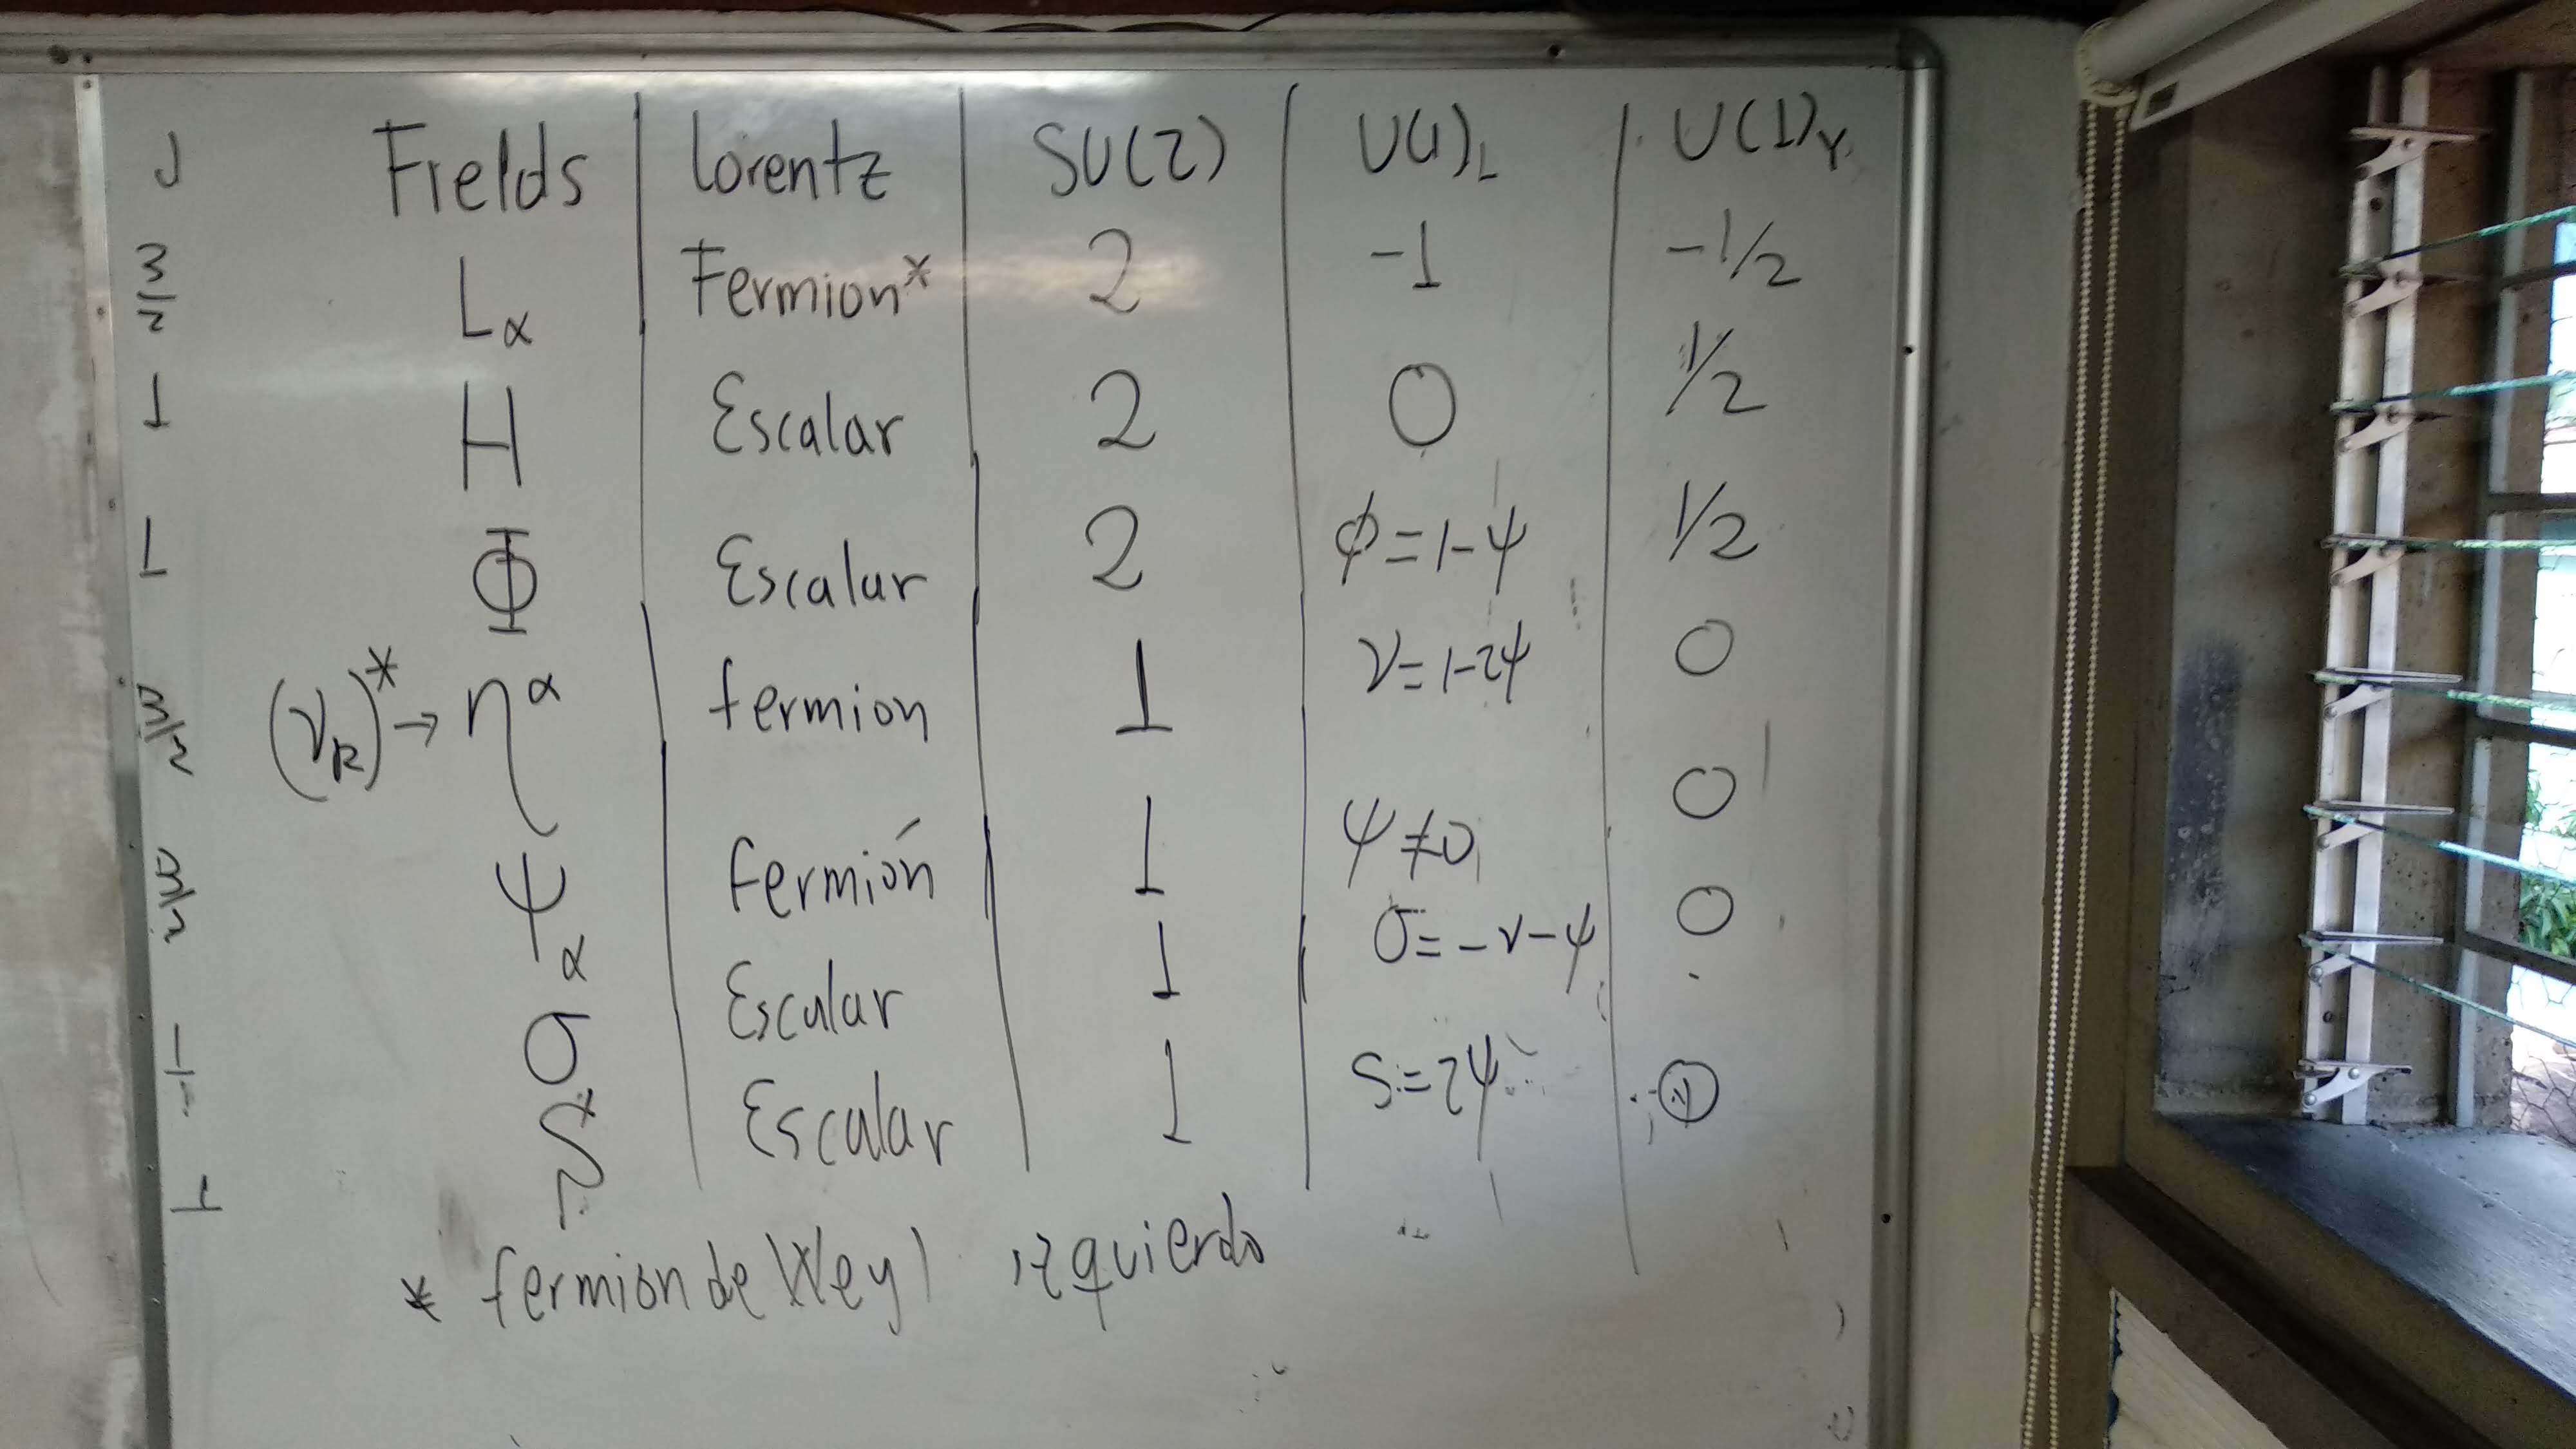
\includegraphics[scale=0.1]{tabla}

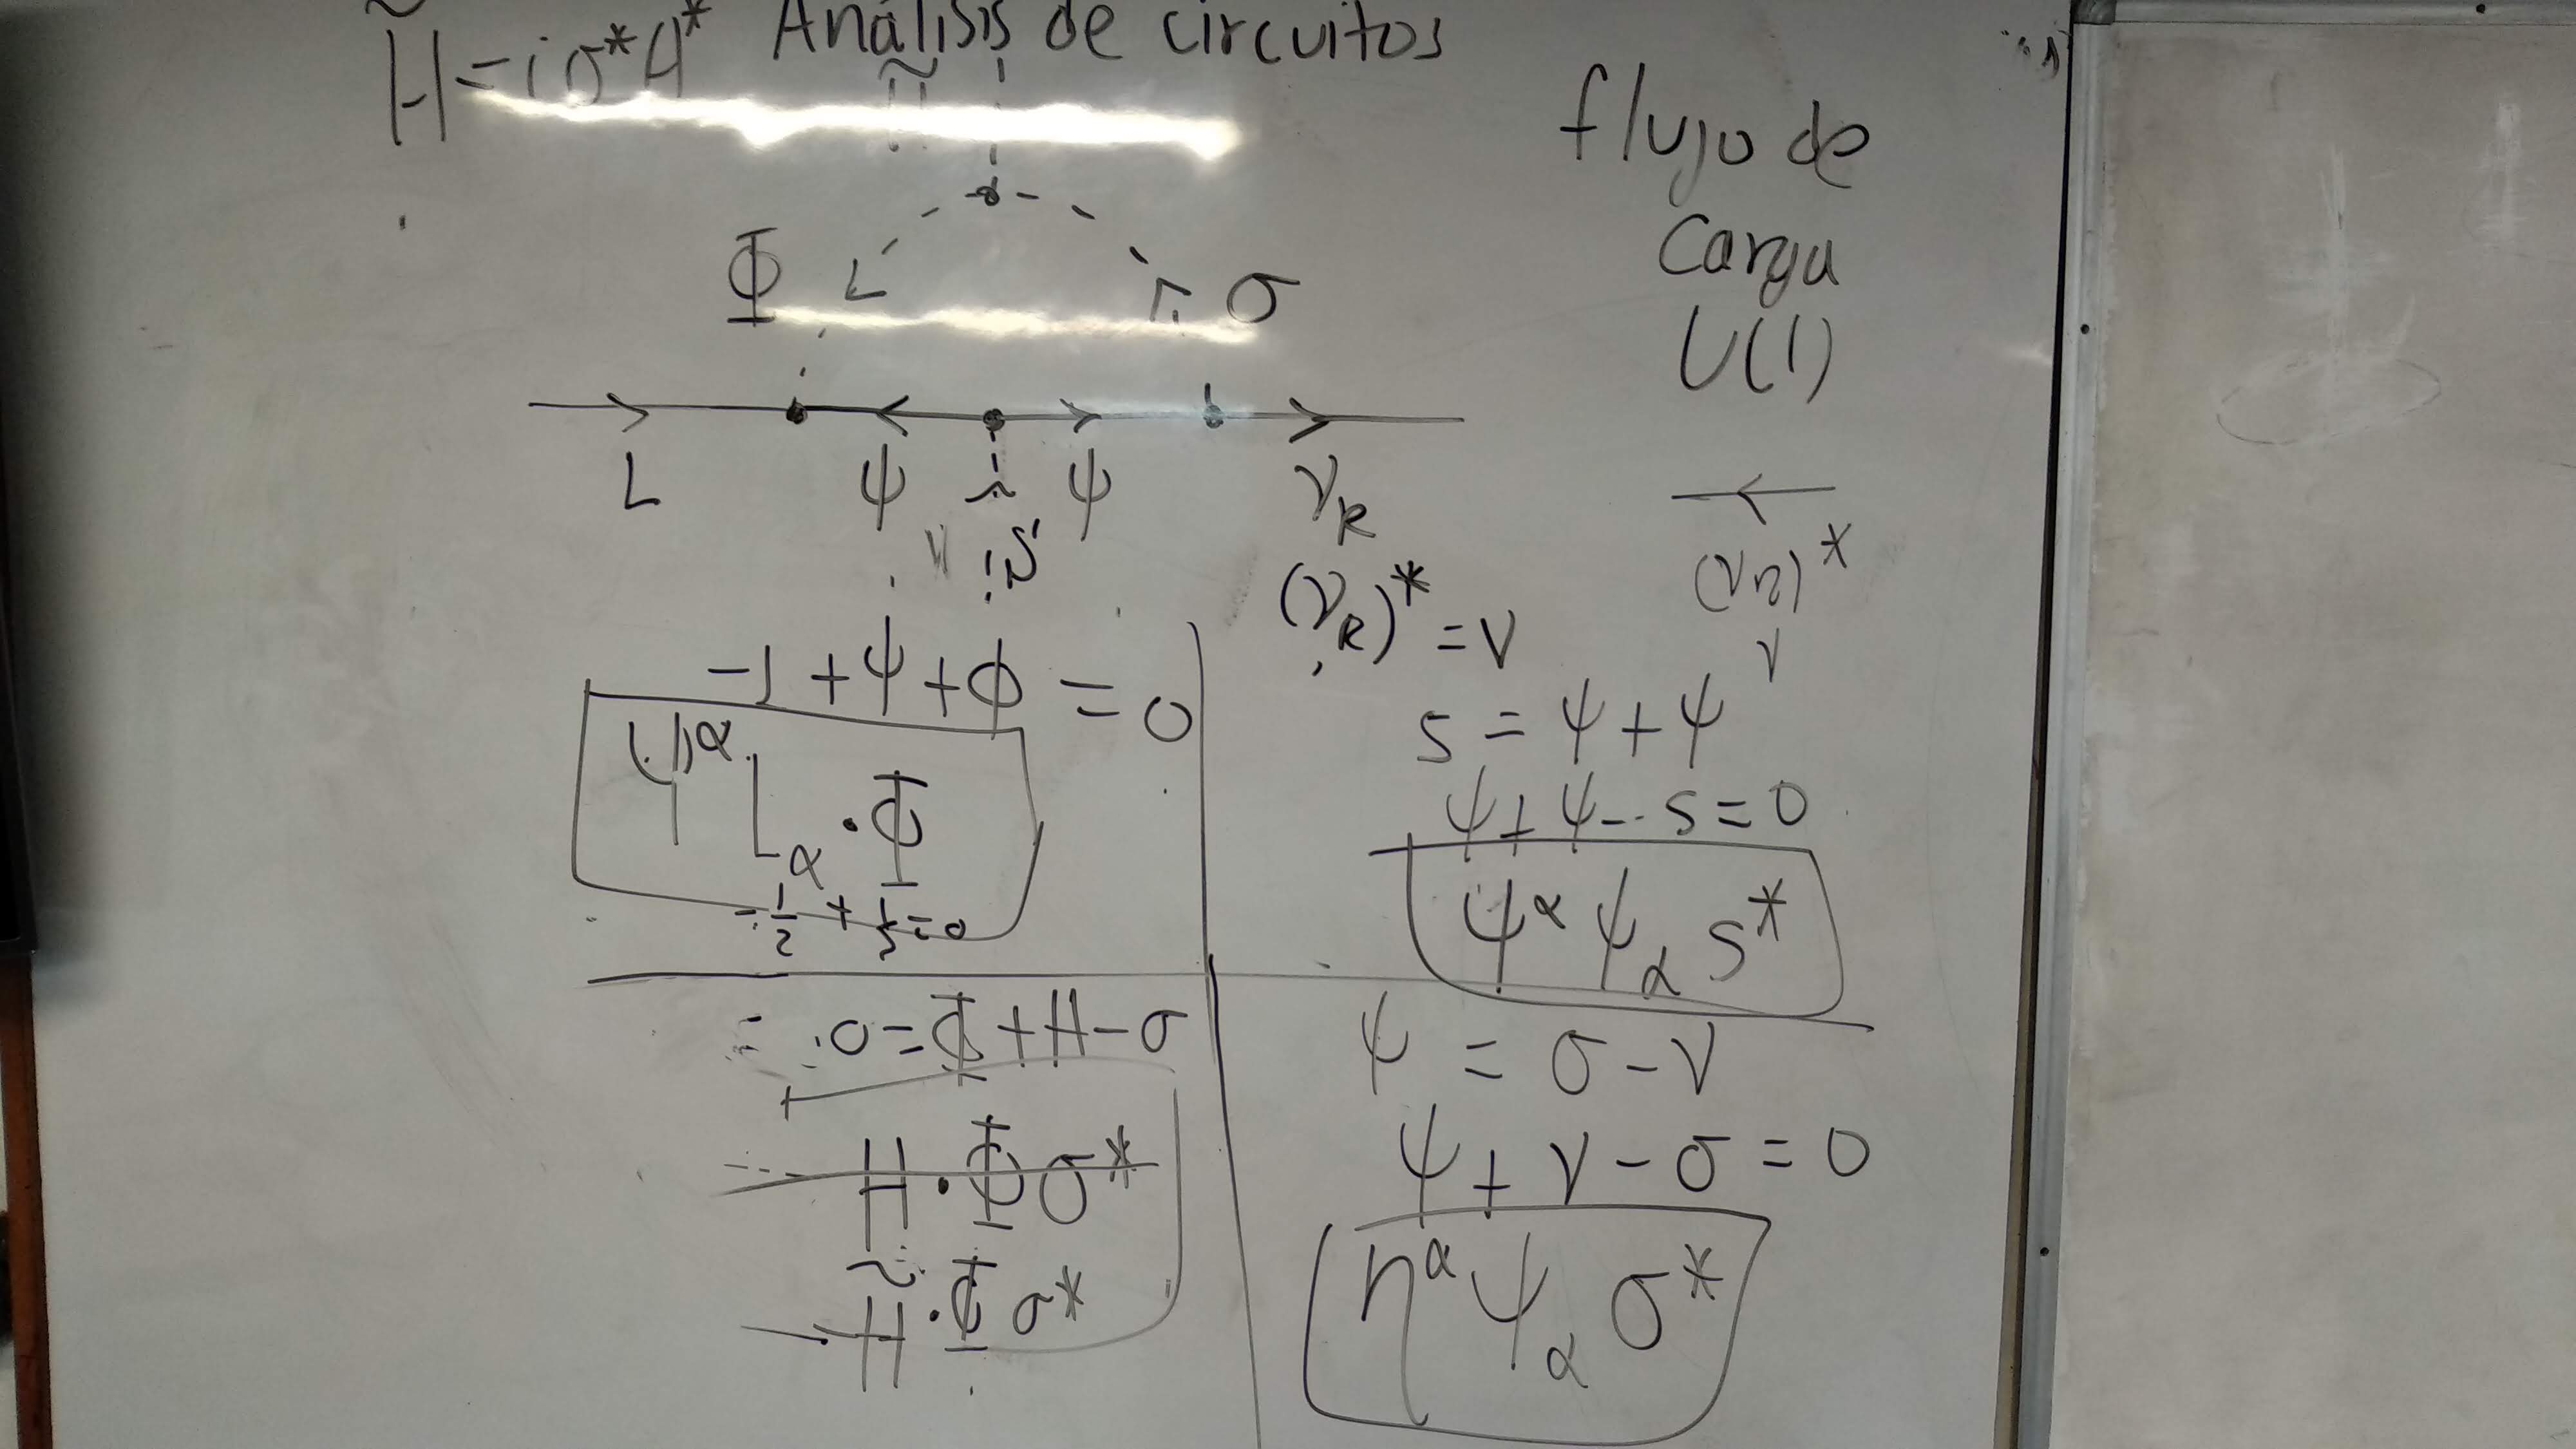
\includegraphics[scale=0.1]{circuito}


\section{Productos escalares}

\section{Diagramas de flujos de cargas}



%%% Local Variables: 
%%% mode: latex
%%% TeX-master: "fullnotes"
%%% ispell-local-dictionary: "castellano8"
%%% End: